
\documentclass[11pt]{amsbook}
\usepackage[turkish]{babel}

\usepackage{../Ceyhun}	
\usepackage{../amsTurkish}


\usepackage{lipsum}



\begin{document}
\hPage{058}
da daha az bire eşit teriminin bulunmasıdır.

	\begin{definition}
		$O_{nj}$ altmatrisine iliskin ayrıtlar, Şekil \ref{fig:2.2.3} de gösterildiği gibi birbirlerine bitişik değildir.\\
		$A_{ij}$ matrisindeki herhangi bir dizekte h sayıda bire
		\begin{figure}[h] \centering 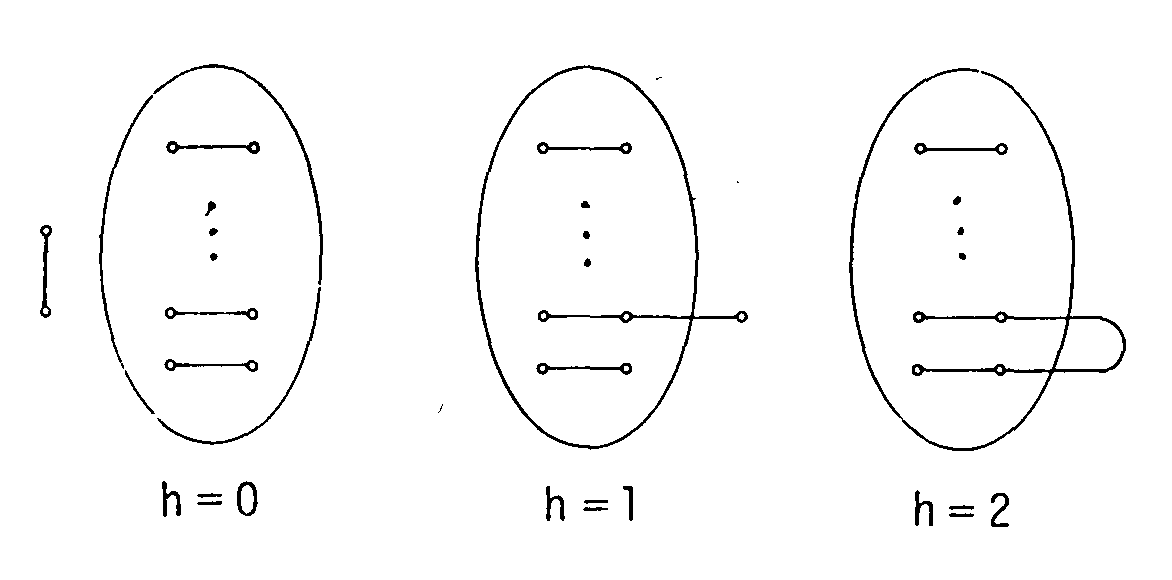
\includegraphics[width=0.9\textwidth,keepaspectratio=true]{images/ceyhun-058-fig01}\caption{ Teorem 2.2.1 in açıklanması} \label{fig:2.2.3} \end{figure}
	\end{definition}
	
	eşit terimin bulunması, bu dizeğe ilişkin ayrıtın $O_{nj}$ altmarisine ilişkin ayrıtlardan h kadarına bitişik olması anlamına gelmektedir.Bu gözlem, 
	Şekil \ref{fig:2.2.3} de gösterildiği gibi h nin, 

	
		$0\leq h \leq 2$
	
	eşitsizliğini sağlamasını gerektirecektir.

\end{document}  

